%%%%%%%%%%%%%%%%%%%%%%%%%%%%%%%%%%%%%%%%%
% Masters/Doctoral Thesis 
% LaTeX Template
% Version 2.5 (27/8/17)
%
% This template was downloaded from:
% http://www.LaTeXTemplates.com
%
% Version 2.x major modifications by:
% Vel (vel@latextemplates.com)
%
% This template is based on a template by:
% Steve Gunn (http://users.ecs.soton.ac.uk/srg/softwaretools/document/templates/)
% Sunil Patel (http://www.sunilpatel.co.uk/thesis-template/)
%
% Template license:
% CC BY-NC-SA 3.0 (http://creativecommons.org/licenses/by-nc-sa/3.0/)
%
%%%%%%%%%%%%%%%%%%%%%%%%%%%%%%%%%%%%%%%%%

%----------------------------------------------------------------------------------------
%	PACKAGES AND OTHER DOCUMENT CONFIGURATIONS
%----------------------------------------------------------------------------------------

\documentclass[
12pt, % The default document font size, options: 10pt, 11pt, 12pt
%oneside, % Two side (alternating margins) for binding by default, uncomment to switch to one side
spanish, % ngerman for German
% Double spacing might be required for Galileo *CHECK* - it is required
doublespacing, % Single line spacing, alternatives: onehalfspacing or doublespacing
%draft, % Uncomment to enable draft mode (no pictures, no links, overfull hboxes indicated)
%nolistspacing, % If the document is onehalfspacing or doublespacing, uncomment this to set spacing in lists to single
liststotoc, % Uncomment to add the list of figures/tables/etc to the table of contents
%toctotoc, % Uncomment to add the main table of contents to the table of contents
%%%%% Required by Galileo Uni formatting
parskip, % Uncomment to add space between paragraphs
%%%%%
%nohyperref, % Uncomment to not load the hyperref package
headsepline, % Uncomment to get a line under the header
%chapterinoneline, % Uncomment to place the chapter title next to the number on one line
%consistentlayout, % Uncomment to change the layout of the declaration, abstract and acknowledgements pages to match the default layout
]{MastersDoctoralThesis} % The class file specifying the document structure

\usepackage[utf8]{inputenc} % Required for inputting international characters
%\usepackage[T1]{fontenc} % Output font encoding for international characters
\usepackage{textcomp}

\usepackage{mathpazo} % Use the Palatino font by default

\usepackage[style=apa]{biblatex} % backend is *biber* set your editor to use that

\addbibresource{thesisbib.bib} % The filename of the bibliography

\usepackage[autostyle=true]{csquotes} % Required to generate language-dependent quotes in the bibliography

\usepackage{comment}

\setcounter{secnumdepth}{3} % Para que las subsubsections tengan número

%----------------------------------------------------------------------------------------
%	MARGIN SETTINGS
%----------------------------------------------------------------------------------------

\geometry{
	paper=letterpaper, % Change to letterpaper for US letter
	inner=2.5cm, % Inner margin
	outer=3.8cm, % Outer margin
	bindingoffset=.5cm, % Binding offset
	top=1.5cm, % Top margin
	bottom=1.5cm, % Bottom margin
	%showframe, % Uncomment to show how the type block is set on the page
}

%----------------------------------------------------------------------------------------
%	THESIS INFORMATION
%----------------------------------------------------------------------------------------

\thesistitle{Aplicación de redes neurales recurrentes de aprendizaje profundo a
perfilación de autores de textos anónimos} % Your thesis title, this is used in the title and abstract, print it elsewhere with \ttitle
%\supervisor{Ing. Alí \textsc{Lemus}} % Your supervisor's name, this is used in the title page, print it elsewhere with \supname
\supervisor{Ing. Ronald \textsc{López}} % Your supervisor's name, this is used in the title page, print it elsewhere with \supname
\examiner{} % Your examiner's name, this is not currently used anywhere in the template, print it elsewhere with \examname
\degree{Ingeniería de Sistemas, Informática y Ciencias de la Computación} % Your degree name, this is used in the title page and abstract, print it elsewhere with \degreename
\author{José Jacobo \textsc{Del Valle Girón}} % Your name, this is used in the title page and abstract, print it elsewhere with \authorname
\addresses{} % Your address, this is not currently used anywhere in the template, print it elsewhere with \addressname

\subject{Ciencias de la computación} % Your subject area, this is not currently used anywhere in the template, print it elsewhere with \subjectname
\keywords{} % Keywords for your thesis, this is not currently used anywhere in the template, print it elsewhere with \keywordnames
\university{\href{http://galileo.edu}{Universidad Galileo}} % Your university's name and URL, this is used in the title page and abstract, print it elsewhere with \univname
\department{\href{http://www.galileo.edu/fisicc/carrera/ii/}{Ingeniería de sistemas}} % Your department's name and URL, this is used in the title page and abstract, print it elsewhere with \deptname
\group{\href{http://turing.galileo.edu/}{Turing Laboratory}} % Your research group's name and URL, this is used in the title page, print it elsewhere with \groupname
\faculty{\href{http://galileo.edu/fisicc}{FISICC}} % Your faculty's name and URL, this is used in the title page and abstract, print it elsewhere with \facname

\AtBeginDocument{
\hypersetup{pdftitle=\ttitle} % Set the PDF's title to your title
\hypersetup{pdfauthor=\authorname} % Set the PDF's author to your name
\hypersetup{pdfkeywords=\keywordnames} % Set the PDF's keywords to your keywords
%\hypersetup{urlcolor=blue} % URL color
\hypersetup{colorlinks=false} % URL color
}

\begin{document}

\frontmatter % Use roman page numbering style (i, ii, iii, iv...) for the pre-content pages

\pagestyle{plain} % Default to the plain heading style until the thesis style is called for the body content

%----------------------------------------------------------------------------------------
%	TITLE PAGE
%----------------------------------------------------------------------------------------

\begin{titlepage}
\begin{center}

\begingroup\onehalfspacing

%\textsc{\Large Proyecto de examen privado}\\[0.5cm] % Thesis type
{\scshape\LARGE \authorname\par}\vspace{1.5cm} % Author name

{\huge \bfseries \ttitle\par} % Thesis title

\vspace{1.5cm}


\includegraphics[scale=0.5]{logo.png} % University/department logo

\vspace{1.5cm}

{\scshape\Large \univname\par} % University name
{\scshape\Large Facultad de Ingeniería en Sistemas,}
{\scshape\Large Informática y Ciencias de la Computación\par}

{\scshape \Large \bfseries Guatemala, \the\year \par}

\endgroup
 
\vfill
\end{center}
\end{titlepage}

%----------------------------------------------------------------------------------------
%	DECLARATION PAGE
%----------------------------------------------------------------------------------------

%\begin{declaration}
%\addchaptertocentry{\authorshipname} % Add the declaration to the table of contents
%\noindent I, \authorname, declare that this thesis titled, \enquote{\ttitle} and the work presented in it are my own. I confirm that:
%
%\begin{itemize} 
%\item This work was done wholly or mainly while in candidature for a research degree at this University.
%\item Where any part of this thesis has previously been submitted for a degree or any other qualification at this University or any other institution, this has been clearly stated.
%\item Where I have consulted the published work of others, this is always clearly attributed.
%\item Where I have quoted from the work of others, the source is always given. With the exception of such quotations, this thesis is entirely my own work.
%\item I have acknowledged all main sources of help.
%\item Where the thesis is based on work done by myself jointly with others, I have made clear exactly what was done by others and what I have contributed myself.\\
%\end{itemize}
% 
%\noindent Signed:\\
%\rule[0.5em]{25em}{0.5pt} % This prints a line for the signature
% 
%\noindent Date:\\
%\rule[0.5em]{25em}{0.5pt} % This prints a line to write the date
%\end{declaration}
%
%\cleardoublepage

%----------------------------------------------------------------------------------------
%	QUOTATION PAGE
%----------------------------------------------------------------------------------------
%
%\vspace*{0.2\textheight}
%
%\noindent\enquote{\itshape Thanks to my solid academic training, today I can write hundreds of words on virtually any topic without possessing a shred of information, which is how I got a good job in journalism.}\bigbreak
%
%\hfill Dave Barry

%----------------------------------------------------------------------------------------
%	ABSTRACT PAGE
%----------------------------------------------------------------------------------------

\begin{abstract}
\addchaptertocentry{\abstractname} % Add the abstract to the table of contents
En tiempos de la expansión masiva del campo del aprendizaje profundo y las aplicaciones que cada vez son más, cada contribución y nueva aplicación al campo no sorprenden, mas son bienvenidas. Este trabajo intenta presentar la tarea del perfilamiento de autores como una tarea que puede ser abordad con aprendizaje profundo pero, sobre todo, que puede aplicarse el concepto de \emph{transfer learning} en el área de NLP y en esta tarea en específico de forma exitosa.\ldots

En tiempos de la expansión masiva del campo del aprendizaje profundo y las aplicaciones que cada vez son más, cada contribución y nueva aplicación al campo no sorprenden, mas son bienvenidas. Este trabajo intenta presentar la tarea del perfilamiento de autores como una tarea que puede ser abordad con aprendizaje profundo pero, sobre todo, que puede aplicarse el concepto de \emph{transfer learning} en el área de NLP y en esta tarea en específico de forma exitosa.\ldots

En tiempos de la expansión masiva del campo del aprendizaje profundo y las aplicaciones que cada vez son más, cada contribución y nueva aplicación al campo no sorprenden, mas son bienvenidas. Este trabajo intenta presentar la tarea del perfilamiento de autores como una tarea que puede ser abordad con aprendizaje profundo pero\ldots
\end{abstract}

%----------------------------------------------------------------------------------------
%	ACKNOWLEDGEMENTS
%----------------------------------------------------------------------------------------

\begin{acknowledgements}
\addchaptertocentry{\acknowledgementname} % Add the acknowledgements to the table of contents
Hay muchas personas a quienes agradecer y aunque tal vez no las logre mencionar a todas aca, principalmente quiero decir que le agradezco a todas las personas que en algún momento me apoyaron durante la carrera o durante la elaboración de este trabajo.

Primero debo agradecerle a mis compañeros en la carrera sin quienes no hubiera llegado a donde estoy. En particular a personas como\ldots

Debo agradecerles también a mis supervisores Alí Lemus y Ronald López. Alí por haber apoyado el enfoque académico que quise darle siempre a este trabajo de investigación.
\end{acknowledgements}

%----------------------------------------------------------------------------------------
%	LIST OF CONTENTS/FIGURES/TABLES PAGES
%----------------------------------------------------------------------------------------
\begingroup\onehalfspacing
\tableofcontents % Prints the main table of contents
\endgroup

\listoffigures % Prints the list of figures

\listoftables % Prints the list of tables

%%----------------------------------------------------------------------------------------
%%	ABBREVIATIONS
%%----------------------------------------------------------------------------------------

\begin{abbreviations}{ll} % Include a list of abbreviations (a table of two columns)

\textbf{CNN} & \textbf{C}onvolutional \textbf{N}eural \textbf{N}etwork\\
\textbf{CV} & \textbf{C}omputer \textbf{V}ision\\
\textbf{DL} & \textbf{D}eep \textbf{L}earning\\
\textbf{FIFO} & \textbf{F}irst \textbf{I}n \textbf{F}irst \textbf{O}ut\\
\textbf{GIGO} & \textbf{G}arbage \textbf{I}n \textbf{G}arbage \textbf{O}ut\\
\textbf{LEFTy} & \textbf{L}anguage \textbf{EF}ficient \textbf{T}ext portra\textbf{y}\\
\textbf{LSTM} & \textbf{L}ong \textbf{S}hort \textbf{T}erm \textbf{M}emory\\
\textbf{ML} & \textbf{M}achine \textbf{L}earning\\
\textbf{NLP} & \textbf{N}atural \textbf{L}anguage \textbf{P}rocessing\\
\textbf{QRNN} & \textbf{Q}uasi-\textbf{R}ecurrent \textbf{N}eural \textbf{N}etwork\\
\textbf{RNN} & \textbf{R}ecurrent \textbf{N}eural \textbf{N}etwork\\
\textbf{ULMFiT} & \textbf{U}niversal \textbf{L}anguage \textbf{M}odel \textbf{Fi}ne-\textbf{T}uning\\

\end{abbreviations}

%%----------------------------------------------------------------------------------------
%%	PHYSICAL CONSTANTS/OTHER DEFINITIONS
%%----------------------------------------------------------------------------------------
%
%\begin{constants}{lr@{${}={}$}l} % The list of physical constants is a three column table
%
%% The \SI{}{} command is provided by the siunitx package, see its documentation for instructions on how to use it
%
%Speed of Light & $c_{0}$ & \SI{2.99792458e8}{\meter\per\second} (exact)\\
%%Constant Name & $Symbol$ & $Constant Value$ with units\\
%
%\end{constants}
%
%%----------------------------------------------------------------------------------------
%%	SYMBOLS
%%----------------------------------------------------------------------------------------
%
%\begin{symbols}{lll} % Include a list of Symbols (a three column table)
%
%$a$ & distance & \si{\meter} \\
%$P$ & power & \si{\watt} (\si{\joule\per\second}) \\
%%Symbol & Name & Unit \\
%
%\addlinespace % Gap to separate the Roman symbols from the Greek
%
%$\omega$ & angular frequency & \si{\radian} \\
%
%\end{symbols}

%----------------------------------------------------------------------------------------
%	DEDICATION
%----------------------------------------------------------------------------------------

\dedicatory{Dedicado a mi familia, amigos y a la comunidad científica lingüística} 

%----------------------------------------------------------------------------------------
%	THESIS CONTENT - CHAPTERS
%----------------------------------------------------------------------------------------

\mainmatter % Begin numeric (1,2,3...) page numbering

\pagestyle{thesis} % Return the page headers back to the "thesis" style

% Custom indentation for Galileo University
\setlength\parindent{2em}

% Include the chapters of the thesis as separate files from the Chapters folder
% Uncomment the lines as you write the chapters

% Chapter 1

\chapter{Introducción} % Main chapter title

\label{Chapter1} % For referencing the chapter elsewhere, use \ref{Chapter1} 

%----------------------------------------------------------------------------------------

% Define some commands to keep the formatting separated from the content 
\newcommand{\keyword}[1]{\textbf{#1}}
\newcommand{\tabhead}[1]{\textbf{#1}}
\newcommand{\code}[1]{\texttt{#1}}
\newcommand{\file}[1]{\texttt{\bfseries#1}}
\newcommand{\option}[1]{\texttt{\itshape#1}}

%----------------------------------------------------------------------------------------

\section{Tema principal}

\ttitle.


%----------------------------------------------------------------------------------------

\section{Introducción}

Los campos de \emph{\gls{machine learning}} (aprendizaje de máquinas o aprendizaje artificial) y \textit{\gls{deep learning}} (\gls{aprendizaje profundo}) \parencite{lecun2015deep} no son para nada nuevos, pero se han vuelto una gran sensación en los últimos años, cada vez ganando más popularidad. Los primeros conceptos desarrollados en el campo tienen décadas de antigüedad. La primer \gls{red neuronal} --- la base del modelo a utilizar en este trabajo y la base del campo de Deep Learning --- fue planteada en los años 80 \parencite{werbos1982applications}. ¿Qué, entonces, ha cambiado en los últimos años que ha generado una explosión en el área? La disponibilidad de los datos y la accesibilidad a poder computacional \parencite{jordan2015machine}. Con el surgimiento y la penetración cada vez más alta del internet se han abierto las puertas a una cantidad de datos nunca antes vista.

La revolución de los datos ha llevado a la comunidad científica y a las industrias a recolectar grandes cantidades de datos e información y organizarlos de forma que se puedan interpretar y se pueda obtener valor de la misma.

Los sistemas de Deep Learning necesitan pasar por una fase de aprendizaje (comúnmente llamada fase de \gls{entrenamiento}) y estos modelos tienen la característica de necesitar cantidades masivas de datos para poder generalizar bien lo aprendido. Esto combinado con la explosión de datos ha llevado a que las técnicas tengan un surgimiento en todas las áreas de software, mostrando mucha promesa en algunos campos en específico como \gls{cv} \parencite{hoo2016deep} y en \gls{nlp}.

Conforme ha avanzado el campo se ha determinado que para algunas tareas en específico no se cuenta con la cantidad necesaria para poder obtener un modelo competente. Esto ha llevado al desarrollo de una técnica llamada transfer learning que permite utilizar conocimiento previamente obtenido al resolver una tarea general y aplicarlo a una tarea relacionada mediante proceso de ajuste. Esta fase requiere de una cantidad de datos considerablemente menor, comparado con tener que entrenar un modelo completamente desde cero.

La técnica de transfer learning ha permitido muchos avances en el área de \gls{cv} específicamente \parencite{hoo2016deep}. Este trabajo intenta mostrar que se puede aplicar este concepto en un área distinta, puntualmente el campo de NLP y específicamente en la tarea de \gls{perfilamiento de autores}.

\section{Hipótesis}

La hipotesis que este trabajo pretende abordar es la siguiente: \textbf{La aplicación de transfer learning en la tarea de perfilamiento de autores provee una ventaja en desempeño medible.} Esta se desglosa en los siguientes aspectos:

\begin{itemize}
\item \textbf{Aplicabilidad de deep learning en la tarea}. La hipótesis se basa en el hecho de que conceptos de deep learning sean aplicables a tareas del campo de NLP. En el campo de NLP se ha tenido mucha duda si deep learning tiene la capacidad de penetrar el campo con soluciones eficaces.

\item \textbf{Transfer learning provee ventaja de desempeño en la tarea}. El hecho de mostrar que hay una ventaja implica medir de forma empírica los resultados obtenidos por diferentes técnicas. Con este fin, se utilizarán resultados publicados por investigadores de este campo y se usarán las mismas métricas para que los resultados sean directamente comparables.

\item \textbf{Diferencia en cantidad de datos disponibles}. Se debe fundamentar que la cantidad de datos necesaria para el uso de deep learning es más elevado del que se necesita si se utiliza transfer learning.
\end{itemize}

%-----------------------------------------------------------------------------------------

\section{Objetivo General}

Aplicar conceptos del estado del arte a un problema que ha recibido poca atención en el área de \gls{procesamiento de lenguaje natural} (\gls{nlp}, por sus siglas en inglés). Esto con el propósito de mostrar la capacidad de las redes neuronales recurrentes (\glspl{rnn}) y \textit{\gls{transfer learning}} en la tarea específica.

\subsection{Objetivos específicos}

\begin{itemize}
\item Ser pionero en la aplicación de transfer learning en la tarea específica de perfilamiento de autores en el área de procesamiento de lenguaje natural.
\item Exponer las ventajas y desventajas de utilizar esta tecnología en esta subtarea.
\item Exponer como caso de uso la utilidad de esta aplicación en distintas áreas, como en el mercadeo.
\item Contribuir a la academia en este campo con los resultados obtenidos
\end{itemize}

%----------------------------------------------------------------------------------------

\section{Planteamiento del problema}

En el área de NLP han existido técnicas poderosas por décadas que abusan de algunas suposiciones que no siempre reflejan la realidad y se basan en simples métodos estadísticos que asignan valores a características del texto \parencite{Edmundson1969, kupiec1995trainable}. El campo también ha dependido de \gls{ingenieria de caracteristicas} en los datos, lo cual significa que se realiza un esfuerzos activo y serio en analizar cada sub-tarea a fondo para determinar cuáles son los mejores determinantes de un resultado deseado, p.e. las características principales que determinan la categoría que se le debe asignar a un texto \parencite{aggarwal2012mining}.

En campos como el mercadeo y las ciencias forenses hay una necesidad de identificar textos escritos a los cuales no se les ha atribuido un autor y obtener características de los mismos para poder catalogarlos de forma automática. Esto con el fin de poder, en el caso del mercadeo, orientar mejor la publicidad de ciertos productos a una audiencia apropiada \parencite{aggarwal2012mining}; y, en el área forense, identificar a sospechosos vinculados a algún crimen a partir de un texto anónimo obtenido en el contexto del caso.

Existe fundamento lingüístico del hecho de poder identificar a una persona por su lenguaje, ya sea de manera escrita u oral \parencite{coulthard2004author, louwerse2004semantic}. El concepto de \textit{\gls{idiolecto}} y \textit{\gls{sociolecto}} nos permitirá realizar predicciones de manera precisa.

Después de analizar lo planteado anteriormente, se ve la necesidad de que un sistema automatizado sea capaz de no sólo extraer información de un texto anónimo de forma precisa y confiable, sino de también hacerlo sin necesidad de un agente experto o realizar una ingeniería de características claves para cada posible parámetro que se quiera obtener de los textos.

A partir de esta conclusión los requisitos para este proyecto son los siguientes:

\begin{itemize}
\item Permitir la categorización de textos a partir de diferentes características.
\item Realizar el entrenamiento para obtener los datos de forma rápida y con demandas de hardware modestas.
\item Una vez el entrenamiento esté completo, permitir realizar predicciones sobre textos anónimos con los datos a obtener elegidos.
\item Permitir la automatización de predicciones ofreciendo un servicio web fácil de consultar.
\end{itemize}

\begin{figure}
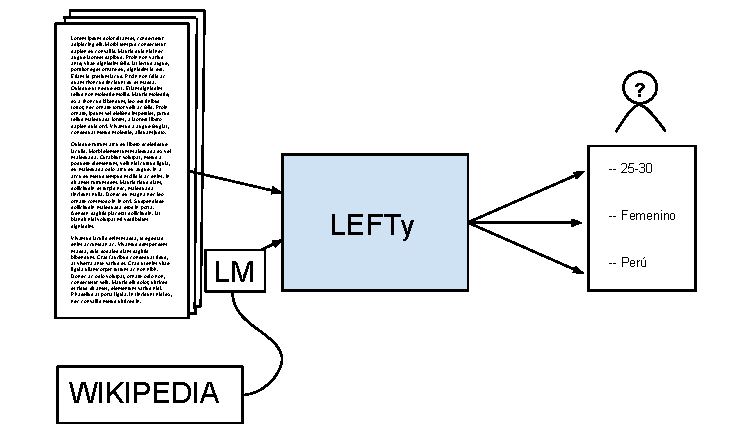
\includegraphics[scale=1.0]{Figures/projectstruct.pdf}
\caption{Estructura del proyecto planteado en este trabajo de investigación. La figura está diseñada para propósitos ilustrativos. \textit{LM} denota el modelo de lenguaje el cual es pre-entrenado con texto de \textit{Wikipedia}, lo cual es un paso previo.}
\label{fig:projstruct}
\end{figure}

La figura \ref{fig:projstruct} muestra la estructura del proyecto planteado, el cual llenaría los requisitos expuestos en esta sección. El flujo de la información tendría la forma ilustrada en la figura y las predicciones mostradas son ejemplos de categorizaciones.

\section{Resumen}

El proyecto deberá tener la flexibilidad de poder adaptarse a las necesidades del caso de uso específico que se le dé y a la vez tener la capacidad predictiva de un modelo del estado del arte. El modelo utilizará tecnologías de Deep Learning por ser la tecnología más prometedora en este campo.






% Chapter 2

\chapter{Trasfondo del aprendizaje profundo} % Main chapter title

\label{Chapter2} % For referencing the chapter elsewhere, use \ref{Chapter1} 

En este capítulo se planteará y se explicará la base teórica del campo del aprendizaje profundo utilizados en este trabajo. Los conceptos descritos a continuación son el fundamento del campo de aprendizaje profundo


\section{Aprendizaje supervisado}

En el área de aprendizaje de máquina (profundo) existen dos tipos básicos de problemas. El tipo se determina dependiendo de el tipo de datos a utilizar para el entrenamiento del modelo.

Cuando los datos --- ya sea información tabulada, imágenes, textos --- no tienen ninguna categoría o ningún valor a predecir y lo que se desea es obtener información no específica, es decir sin tener alguna referencia, se trata de un aprendizaje no supervisado.

Si los datos, por otro lado, tengan una clasificación, llamada etiqueta, asignada, la cual a futuro es el resultado a predecir, los métodos a utilizar son los del aprendizaje supervisado. Debido a que el problema a abordar en este trabajo es un problema de clasificación, el resto del fundamento teórico será basado en el contexto del aprendizaje supervisado.

El aprendizaje supervisado puede entonces ser descrito como una función $f : X \to Y$ donde $X$ representa los datos con los que se alimenta la función, es decir con los que se entrenará el modelo, y $Y$ el resultado a asignado o a predecir.

Para ilustrar el proceso de aprendizaje de máquina profundo se utilizará un caso individual de la función en donde $y$ es el resultado deseado y $f(x) = \hat{y}$ es la función aplicada a un caso específico y $\hat{y}$ representa el resultado obtenido con la función el cual no necesariamente es el resultado deseado y esperado.

\textbf{El objetivo.} En concreto, buscamos una función $f$ que sea la mejor candidata para poder predecir los resultados deseados. Si definimos una función de costo $L(\hat{y}, y)$ que representa, en un valor escalar, la diferencia cuantitativa entre la evaluación de una función $f$ candidata y el resultado real $y$ podemos concluir que el objetivo es encontrar una $f^*$ que cumpla con:

$$f^* = \min_{f \in F} \frac{1}{N} \sum_{i = 0}^{N} L(f(x_i), y_i)$$

Donde $n$ es el número de instancias de los datos para entrenar el modelo; $F$ siendo un conjunto de funciones candidatas.

\textbf{Definiendo las funciones.} La base de todo modelo de aprendizaje profundo es una red neuronal --- cuyo comportamiento será definido en la siguiente sección junto con otros detalles --- y su comportamiento puede ser descrito de la siguiente forma:

$$ f(x_i) = w x_i + b $$

Siendo $x_i$ la instancia $i$ con propósitos de entreno o de predicción. Esto nos dice que $w$ y $b$ serán los parámetros a modificar de una manera sistemática para encontrar la función $f^*$. Con fines de brevedad, la concatenación de $w$ y $b$ serán representados por $\theta$.

La función de pérdida para una predicción obtenida toma la forma del error de la entropía cruzada, es decir:

$$ L(\hat{y_i}, y_i) = y_i log\hat{y_i} + (1 - y_i)log(1 - \hat{y_i}) $$

Teniendo ya la pérdida para una predicción se puede expandir esta idea para obtener la pérdida a través de un conjunto de datos, lo cual resultará muy útil cuando se deba entrenar. Para obtener una aproximación de la perdida sobre un conjunto de datos se podrá utilizar el promedio sobre las perdidas individuales de los datos evaluados:

$$ L(\hat{y}, y) = - \frac{1}{N} \sum_{i = 1}^{N} [y_i log\hat{y_i} + (1 - y_i)log(1 - \hat{y_i})] $$

\textbf{Optimizando la función de costo.} Teniendo entonces una función a minimizar y una cantidad $N$ de datos sobre los cuales se deberá ir encontrando una función $f$ candidata cada vez mejor se recurre al método de el descenso de gradiente. Este método nos permite, utilizando propiedades básicas de las derivadas de las funciones, poco a poco avanzar hasta llegar a un mínimo de la función. Cada nueva función candidata entonces podrá ser derivada de la siguiente forma:

$$ f_i(x_i) = \theta_i x_i $$

Donde
\begin{equation}
\label{eq:sgdupdate}
\theta_{i + 1} = \theta_{i} - \gamma \nabla_{\theta} L(\hat{y_i}, y_i)
\end{equation}

Este proceso de utilizar el descenso de gradiente a través de las instancias nos permite ir minimizando el error de la función hasta poder deducir la función que muestra el menor error.

\textbf{La tasa de aprendizaje.} La velocidad de convergencia de este proceso dependerá en gran parte en $\gamma$ que representa la tasa de aprendizaje, es decir, es la ponderación que se le da al gradiente cuando se propone la nueva función. Un $\gamma$ muy alto arriesga una divergencia debido a que podría oscilar alrededor de un mínimo sin nunca poder converger en él. Un $\gamma$ muy bajo, por el otro lado, puede resultar en un aprendizaje muy lento, lo cual puede llevar a un resultado no óptimo. Este concepto será importante en capítulos posteriores de este trabajo.

\section{Redes neuronales}

Las redes neuronales son el modelo base para el aprendizaje profundo. Con ayuda de el concepto de las redes neuronales especificaremos más acerca de la función $f$ que hasta ahora ha permanecido general, únicamente sabiendo que es derivable. Hay diferentes tipos de redes neurales en el campo y en este trabajo se abordarán únicamente las redes neuronales estándar y las recurrentes.

\subsection{Redes neuronales estándar}

\begin{figure}
	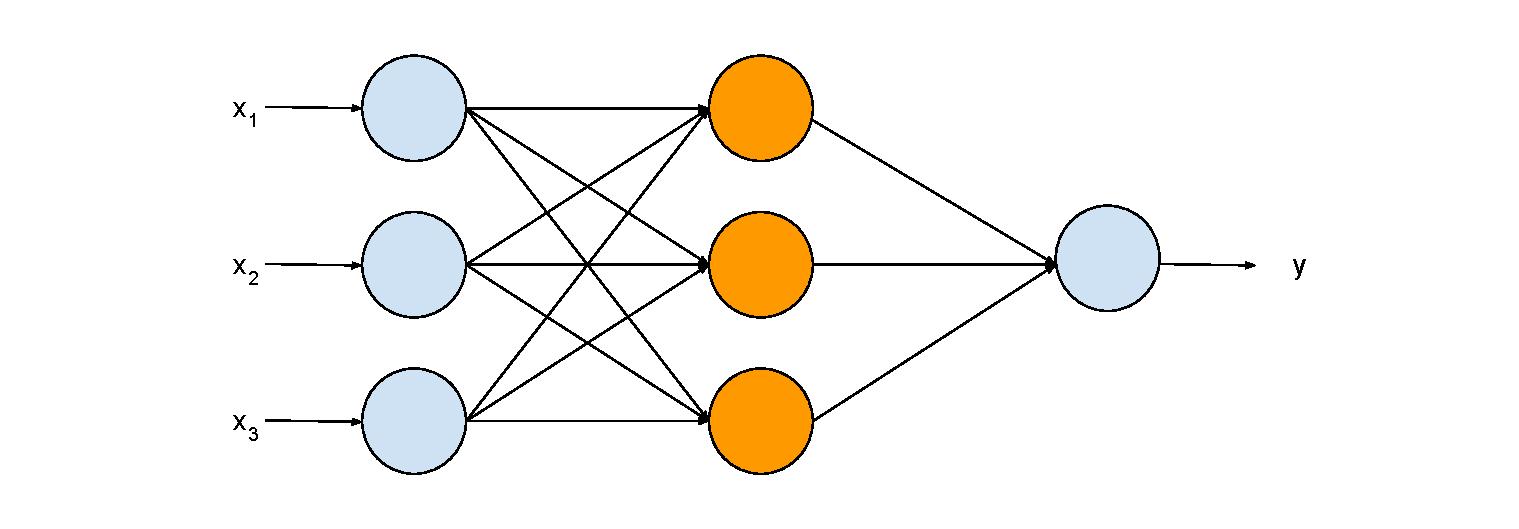
\includegraphics[scale=.6]{Figures/standardnn.pdf}
	\caption{Una red neuronal estándar con una capa oculta, la cual tiene 3 unidades neuronales. La red está completamente conectada y tiene 3 nodos de entrada.}
	\label{fig:standardnn}
\end{figure}

\textbf{Inspiración.} Estas redes neuronales fueron basadas en comportamientos biológicos y reflejan un comportamiento similar a la comunicación de neuronas que se aprecia en la naturaleza. La entrada de datos en una neurona es procesada y alimentará a la siguiente neurona y así sucesivamente hasta haber recorrido toda la red. La redes neuronales no son sucesiones directas y lineales de neuronas; las redes están divididas en capas, las cuales pueden contener más de una unidad. En una red completamente interconecteda, como la que se aprecia en la figura \ref{fig:standardnn}, conecta a todas las unidades de una capa con todas las unidades de la siguiente. Así como las neuronas en la naturaleza, las neuronas en una red neuronal tienen una unidad o célula principal, axones y su conexión es llamada sinapsis.

\textbf{Propagación hacia adelante.} En las redes neurales es el proceso del flujo de la información a través de la red y sus funciones hasta obtener un resultado. En el caso de una red neuronal típica, este proceso significa que la salida de una neurona en una capa alimenta parcialemente a las de la capa siguiente. La función a utilizar por cada unidad individual es una regresión linear simple que puede ser descrita como $f(x) = W x$, es decir, una matriz de parámetros a multiplicarse con los datos de entrada a la neurona. Adicional a esto se maneja una función de activación para el resultado de esa multiplicación, la cual es una no linearalidad a cada elemento resultante (p.e. $\tanh$). De esto se concluye que para, por ejemplo, obtener el resultado de una neurona en la cuarta capa se tiene que
\begin{equation}
\label{eq:feedfwdeq}
f(x) = W_4 \sigma(W_3 \sigma (W_2 \sigma(W_1 x)))
\end{equation}

Donde $W_4$ es una matriz de parámetros de la cuarta capa, $W_3$ es una matriz de parámetros de la tercera capa, y así sucesivamente, y $x$ representa los datos de entrada.

%Figura demostrando fwd y back prop
\begin{figure}
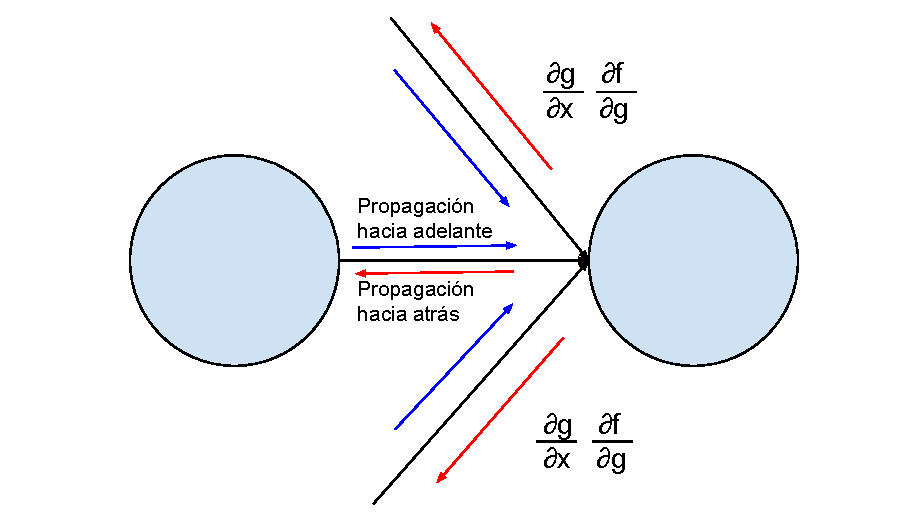
\includegraphics[scale=0.8]{Figures/backprop.pdf}
\caption{En azul podemos ver la dirección del flujo de información durante la propagación hacia adelante. En rojo podemos ver que la dirección se invierte para la propagación hacia atrás y que lleva los gradientes necesarios para propagar el error después del entrenamiento.}
\label{fig:backprop}
\end{figure}


\textbf{Propagación hacia atrás.} Ya que está presente un mecanismo para evaluar el conjunto de funciones que representa cada unidad de la red, debemos tener un mecanismo para optimizar los parámetros que definen cada función. La propagación hacia atrás se encarga de esto utilizando el concepto previamente descrito como el descenso de gradiente. Para realizar la propagación hacia atrás se aplica la regla de la cadena la cual establece que si $\frac{\partial f(g(x))}{\partial x} = \frac{\partial g}{\partial x} \frac{\partial f}{\partial g}$. Notemos que la función que se quiere derivar toma una forma similar a la que tenemos en la ecuación \ref{eq:feedfwdeq}, con la adición de que $g(x)$ es una función que anida aún más funciones. Para obtener la optimización de los parámetros podemos derivar en dirección hacia atrás propagando la mejora que se propone con el gradiente.

\subsection{Redes neuronales recurrentes}

% Figura con una LSTM y su descripcion


Este tipo de redes tienen la peculiaridad que se alimentan no solamente de los resultados de las funciones de activación de las capas anteriores sino también del resultado para la instancia previamente evaluada --- para datos evaluados en $t - 1$ la definición sería $h_t = f_{\theta}(h_{t-1}, x_t)$. Este tipo de estructura es aplicado a conjuntos de datos secuenciales como lo es el procesamiento de textos --- textos cuya representación consiste en una secuencia de palabras representadas de forma vectorial --- y procesamiento de secuencias de señales.

Se debe aclarar para esta estructura de red neural también existen distintos tipos. El subtipo relevante para este trabajo de investigación es la red LSTM (Long Short Term Memory -- memoria corta a largo plazo). Estas tienen un dato en memoria en cada una de las unidades de la red. Los parámetros con los que se decide si se sobreescribe lo que está en memoria en esa celda en ese momento pueden ser entrenados también con el mecanismo de propagación hacia atrás.

Los mecanismos de propagación hacia adelante y hacia atrás permanecen iguales pero se deberán tomar en cuenta adicionalmente las puertas (\textit{gates}) con sus funciones de activación. Estas son definidas como la función sigmoide, la cual es continua y tiene un contradominio de $[0,1]$ lo cual la hace derivable en todos sus puntos.

\section{Generalización de una red neuronal}

Una red neuronal aprende a elegir una función que minimice el costo de evaluar un conjunto de datos. Intuitivamente podemos ver que este proceso lleva a que la red aprenda características de los datos que está utilizando y poco a poco aprenda a predecir este conjunto de datos de manera más precisa. Las palabras claves son \textit{este conjunto de datos}, es decir se habla de que la red aprende sobre un conjunto limitado de datos y fuera de él no hay garantía de que sepa algo. Para que el modelo pueda generalizar lo aprendido con estos datos existen distintos mecanismos. En esta sección se explicarán dos de estos conceptos.

\textbf{Cantidad de datos.} La cantidad de datos utilizados para entrenar un modelo influye mucho en su capacidad de generalizar. Mientras más datos se tengan, mayor será la posibilidad de generalizar, esto con la condición que la data sea diversa y representativa del problema real. La explicación de esto se puede ilustrar llevando el concepto a sus extremos y con un ejemplo sencillo. Suponiendo que se quiere aprender a definir el conectivo lógico \textbf{\textit{and}}. Si se provee solamente un ejemplo de cómo funciona este operador, la red no sabrá que hacer cuando los valores de entrada varíen. Por el otro lado si le alimentamos todas las combinaciones posibles, la red deberá ser capaz de aprender todo el contexto del problema.

\textbf{Término de regularización.} Esta técnica es muy esencial cuando se lidia con modelos de aprendizaje profundo. Consisten en agregar un término de regularización a la función de predicción que se está optimizando. La función entonces tendrá la forma siguiente: %hacer referencia a la misma de antes

$$f^* = \min_{f \in F} \frac{1}{N} \sum_{i} L(f(x_i), y_i) + \sum_{j} \lambda(w_j^2)$$

Esto funciona ya que limita el crecimiento de los parámetros, el cual desenfrenado podría causar una explosión de gradiente. Esto tiene como consecuencia que el modelo sea incapaz de converger.

\section{Proceso general al aplicar una red neuronal}

Un proyecto de aprendizaje profundo con redes neuronales lleva por lo general el mismo conjunto de pasos para poder llegar a un resultado cercano a lo óptimo. Los pasos a seguir son los siguientes:

\begin{itemize}
\item \textbf{Obtención de datos:} Dependiendo del problema a resolver estos datos podrán tomar distintas formas y los métodos para obtenerlos podrán variar en gran forma. Para que una red neuronal pueda generalizar de forma exitosa lo aprendido durante la fase de entrenamiento es importante tener una muestra representativa del escenario real del problema a resolver y tener una cantidad grande de datos. Métodos comunes incluyen recolección y etiquetación manual, descarga de \textit{corpora} de internet, \textit{scraping} de la web.

\item \textbf{Análisis y preparación de los datos:} Los datos obtenidos en el primer paso pueden llegar a tener características mínimas no deseadas, las cuales pueden añadir ruido a la representación que estos datos dan. Debido a esto es importante tratar los datos de manera que se eliminen datos que sesguen mucho la data, datos faltantes, datos con formato inconsistente, e incluso considerar la posibildad de eliminar características completas. En esta fase también se separarán los datos en distintos segmentos que después serán útiles para determinar la eficacia del modelo resultante. Estos segmentos son los datos de \textit{entrenamiento, validación} y \textit{prueba}. La proporción de cada uno de estos puede variar y lo recomendado es que la distribución de cada uno de ellos sea la misma. De no ser posible esto, hacer que al menos los segmentos de validación y prueba tengan la misma distribución.

\item \textbf{Diseño de modelo:} En este campo hay una gran variedad de opciones, en especial si no se limitan estas opciones al aprendizaje profundo ya que existen herramientas de distintos tipos para poder modelar un sistema. En el caso del aprendizaje profundo también se deberán tomar decisiones importantes con respecto al modelo a utilizar. En concreto se deberá elegir el tipo de red neuronal a utilizar como también su estructura. En esta fase se definirán de forma preliminar detalles como el número de capas a utilizar en la red y el número de unidades por cada una de las capas.

\item \textbf{Optimización de hiper-parámetros:} Esta fase estará muy relacionada a la siguiente ya que se utilizan los mismo mecanismos para determinar los resultados preliminares. Para elegir los mejores hiper-parámetros para un modelo en específico se deberá evaluar los datos variando sus valores y obteniendo resultados preliminares. Esto se deberá hacer utilizando una matriz aleatoria para los distintos hiper-parámetros con el fin de optimizar el tiempo de ejecución de esta fase.

\item \textbf{Entrenamiento del modelo:} En esta fase se optimizarán los parámetros de la red para que esta sea capaz de modelar el problema y poder realizar predicciones. En esta fase se aplicarán de forma iterativa las fases de propagación hacia adelante y hacia atrás hasta llegar a una convergencia. Si se cuenta con tiempo limitado, se deberá elegir un resultado que sea suficientemente satisfactorio y se detendrá el entrenamiento en ese punto.

\item \textbf{Validación de resultados:} Durante esta fase se hará uso de los datos segmentados para validación. Sobre estos datos se aplicará el modelo en su modalidad de propagación hacia adelante únicamente con lo que se obtendran predicciones las cuales se podrán comparar con los valores reales de los datos. El fin de evaluar el modelo en datos que no están presentes en los datos de entrenamiento es determinar el poder de generalización del modelo.

\end{itemize}

Los pasos de entrenamiento y validación de resultados podrán repetirse las veces que sean necesarias variando parámetros y evaluando los tipos de errores para mejorar los resultados.

% Chapter 3

\chapter{Transferencia de aprendizaje} % Main chapter title

\label{Chapter3} % For referencing the chapter elsewhere, use \ref{Chapter1} 

Un concepto esencial para este trabajo y para toda el área de aprendizaje profundo es la capacidad de transferir aprendizaje adquirido previamente de un problema poco acotado y poder lograr aprovechar este aprendizaje en problemas más acotados permitiendo así que las demandas de recursos como datos y tiempo de ejecución tengan más holgura. Se obtienen mejores resultados transfiriendo aprendizaje de un modelo que cuando se inicializan los pesos de los parámetros de al red aleatoriamente \parencite{Erhan:2010:WUP}.

\section{Concepto de transferencia}

Las redes neuronales capturan diferente información en sus capas \parencite{yosinski:2014, zeiler2014visualizing} y la forma en que difieren permite transferir conocimiento a través de redes entrenadas para diferentes tareas. En las primeras capas se aprende información bastante abstracta con respecto a la tarea y conforme se avanza en la profundidad de la red se vuelve más específica la información que se va aprendiendo. Debido a esto se puede utilizar lo aprendido en las primeras capas para otra tarea del mismo dominio.

\begin{figure}
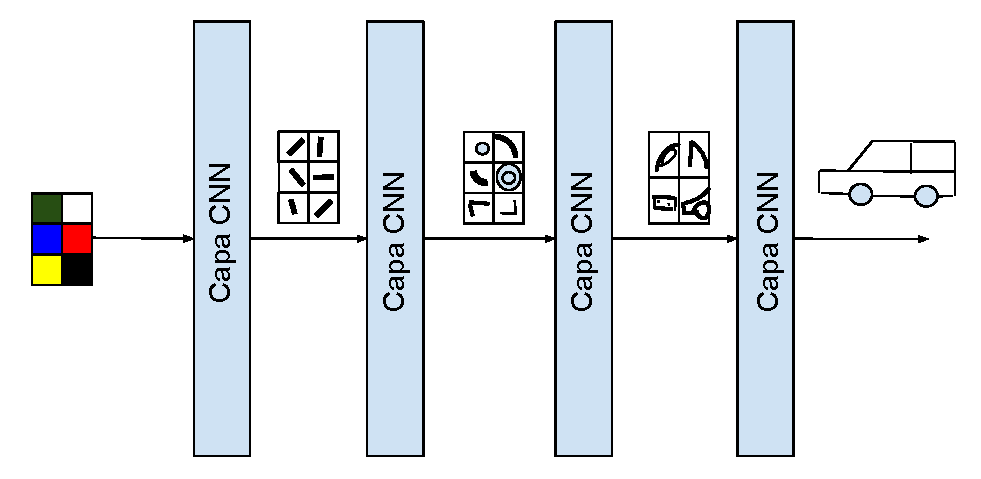
\includegraphics[scale=1]{Figures/learnbylayer.pdf}
\caption{Ejemplo ilustrativo de lo que podría aprender una red profunda de visión artificial para la detección de vehículos.}
\label{fig:learnbylayer}
\end{figure}

\textbf{Ejemplo ilustrativo.} En una red neuronal cuya tarea es en el área de visión artificial las primeras capas comienzan a entender conceptos de orillas horizontales o verticales; las siguientes capas podrán entender qué son esquinas circunferencias; las siguientes capas podrán entender límites de objetos; etc.

La información en las primeras capas de una red neuronal de visión artificial puede llegar a ser muy útil sin importar la tarea final o qué tan acotada esté. Por esta razón es posible tomar un modelo pre-entrenado en una tarea general, remover su capa final --- la cual determina el resultado final de esa tarea en específico --- y continuar con el proceso de entrenamiento con datos de la tarea más acotada y permitir que las nuevas capas no entrenadas aprovechen los conceptos de las capas anteriores para poder ellas tener le poder de predecir usando esa información los resultados correctos.



\section{Aplicación en otras áreas}
%Incluir trabajos relacionados
Para tener el contexto acerca de este concepto crucial para este trabajo debemos explorar otras áreas del aprendizaje profundo, en particular el área de visión artificial (computer vision en inglés). Este campo fue el que llevó a la explosión del aprendizaje profundo en el 2012 cuando una red denominada AlexNet dominó la competencia de clasificar el dataset ImageNet \parencite{deng2009imagenet}.

\textbf{ImageNet.} Este proyecto es una colección masiva de imágenes que están debidamente etiquetadas con cuadros encerrando los objetos detectados en una imagen. Debido a la cantidad exagerada de categorías y objetos encontrados en las imágenes y también la cantidad en sí de imágenes, se organiza un concurso de software todos los años para determinar cuál modelo es el mejor en visión artificial. Cuando en el 2012 una red de aprendizaje profundo ganó el concurso se generó motivación en explorar este campo más a fondo.

Esta tarea llegó a ser el estándar para poder determinar si un modelo podía \emph{ver} a nivel general. ¿Qué significa esto? La tarea de ver es una tarea muy basta y bastante general. Hay muchas características por considerar lo cual aumenta la complejidad de este problema.

% incluir ilustracion de imagenet aca

En CV existen muchas más tareas más acotadas que ver. Para estas sería muy útil poder utilizar información previamente aprendida con la finalidad no necesitar muchos datos para la tarea más específica. Por su misma naturaleza tendrá menos datos de entrenamiento.

\section{Aplicación en NLP}

Hasta el año 2018 no se había aplicado la transferencia de aprendizaje en el área de NLP, pero eso cambió después de trabajos pioneros \parencite{peters:2018, howard2018, devlin2018bert} la técnica muestra promesa. Se podría decir que el momento ImageNet ha llegado a NLP y el progreso ha sido de crecimiento explosivo.

La tarea general en NLP para tener un modelo base ha sido la tarea del modelo de lenguaje \parencite{howard2018}. Un modelo de lenguaje es el que intenta predecir la próxima palabra tomando en cuenta las palabras mandadas como argumento al modelo. En textos de temas específicos esto podrá resultar ser un tanto más fácil debido al vocabulario más limitado y por tener acotado el tema. Idealmente para poder tener una generalización poderosa y que puede aportar en tareas de muy distintos campos, se debe tener un modelo de lenguaje aprendido de un corpus de datos amplio y la cantidad de textos deberá ser masiva.

Un corpus que cumple con los requisitos mencionados sería la versión de Wikipedia en el lenguaje deseado. La enciclopedia virtual abarca muchos temas y tiene una diversidad incomparable de vocabulario. Este incluso deberá ser limitado a una cantidad $T$ de tokens. En futuros trabajos se deberá explorar la posibilidad de utilizar distintos corpora.

El modelo de lenguaje es entrenado usando redes neuronales recurrentes en alguna variante que se considere prudente. Una red LSTM o una QRNN \parencite{bradbury2016} son ideales para propósitos de este trabajo y han mostrado los mejores resultados del estado del arte en modelos de lenguaje.

\subsection{ULMFiT}

Esta técnica expuesta originalmente por \textcite{howard2018} en su curso de aprendizaje profundo fue publicado para plantear el algoritmo de forma más formal y con estudios de ablación demostrar que cada aspecto de los pasos es esencial para obtener los mejores resultados. La técnica de ULMFiT se divide en dos fases \parencite{howard2018} las cuales se explicarán a continuación.

\subsubsection{Afinación de modelo de lenguaje}
\label{lmftune}

Esta fase de la técnica consiste en tomar el modelo de lenguaje general y afinarlo para que esté orientado a la tarea final específica con la que se trabajará. Esto se logra utilizando los datos de la tarea final para formar un texto sobre el cual se terminará de entrenar. Para lograr este afinamiento de la mejor manera se utilizan diferentes técnicas.

\textbf{Afinamiento discriminatorio.} Esta técnica llamada \emph{discriminative fine-tuning} en el artículo original consta en usar una tasa de aprendizaje diferente a lo largo de las capas. Es decir, cada capa tiene asignada una tasa de aprendizaje distinta. Se define entonces que los parámetros serán divididos en ${\theta^1, \ldots, \theta^L}$ donde $L$ es el número de capas y $\theta^t$ es el conjunto de parámetros de la capa $l$. La actualización de los parámetros entonces, basado en la ecuación \ref{eq:sgdupdate}:

\begin{equation}
\label{eq:discupdate}
\theta_t^l = \theta_{t-1}^l - \gamma^l \nabla_{\theta} L(\theta)
\end{equation}

\textbf{Tasa de aprendizaje en triangulo inclinado.} Llamado \emph{slanted triangle learning rates} en el artículo original. Durante el recorrido a través de los datos se varía la tasa de aprendizaje tal que su valor aumente durante las primeras $cut$ instancias donde,

$$ cut = \lfloor T \cdot cut\_frac \rfloor$$

$cut\_frac$ es la fracción de datos que queremos sean aprendidos con el crecimiento de la tasa de aprendizaje. Después de que este porcentaje es alcanzado la tasa de aprendizaje deja de incrementar en valor y empieza a disminuir de forma menos acelerada hasta que se termina de iterar sobre los datos de entrenamiento.

\subsubsection{Afinación de modelo a tarea de clasificación}

Para afinar el modelo de la tarea de clasificación se deberá aplicar el mismo pre-procesamiento en cuanto a tokens de vocabulario. Tener el modelo pre-entrenado y afinado permite obtener resultados bastante precisos sin necesidad de tener muchos datos de entrenamiento para la tarea específica.

Para el afinamiento de este modelo se aplican los conceptos desarrollados en la sección \ref{lmftune}. Adicionalmente se utiliza una técnica que previene la pérdida de conocimiento.

\textbf{Descongelamiento gradual.} Llamado \emph{gradual unfreezing} en el artículo original. Esta técnica es de las más importantes. El concepto de transferencia de aprendizaje se basa en no perder conocimiento aprendido desde la tarea general original. Al refinar un modelo completamente se toma un gran riesgo de \emph{olvidar} vasta información. Esta técnica propone congelar los pesos de todas las capas e ir descongelando una por una y después ajustar y entrenar todas las capas descongeladas. Iterando sobre esto hasta que ya no hay capas por descongelar y se termina de afinar el modelo completo.

\subsection{Modelo de lenguaje bidireccional}

Existe la posibilidad de volver el modelo de lenguaje en un modelo bidireccional \parencite{howard2018}. Esto se puede hacer de forma manual al revertir el orden de los textos en el corpus y entrenar de la misma forma. Al tener ambos modelos listos se pueden promediar los resultados de las predicciones de cada modelo para obtener una predicción final.

Esto ha sido denominado como un modelo bidireccional poco profundo o superficial \parencite{devlin2018bert}. Esto no debido a que no es un modelo de aprendizaje profundo, sino que la representación en ambas direcciones no está presente en el modelo sino se logra con el resultado de dos modelos unidireccionales independientes.

% Chapter 4

\chapter{Datos utilizados}

\label{Chapter4} % For referencing the chapter elsewhere, use \ref{Chapter1} 

``On two occasions I have been asked, "Pray, Mr. Babbage, if you put into the machine wrong figures, will the right answers come out?" ... I am not able rightly to apprehend the kind of confusion of ideas that could provoke such a question.''

\hfill ---Charles Babbage, Passages from the Life of a Philosopher

El concepto de \emph{garbage in, garbage out} (basura para adentro, basura para afuera) es muy conocido e indica como un modelo, análisis, etc. es limitado en su capacidad por los datos que se usen para alimentarlo.

En proyectos de aprendizaje artificial se dice que el 80\% del tiempo se deberá usar para la limpieza y tratado de datos. Esta proporción no se mantiene cuando se lidia con modelos de aprendizaje profundo en muchos casos pero el principio es el mismo: no se debe subestimar la importancia de los datos y su integridad.


\section{Pre-procesamiento de datos}

\subsection{Datos tabulares}

\begin{table}
\centering
\begin{tabular}{c c c c | c c}
CORRELATIVO & Edad & Género & País & Sueldo & Moneda \\
\hline
1 & 24 & F & GT & 3500 & GTQ \\
2 & 145 & M & Perú & 100,500 & Soles \\
3 & 35 & N/A & .es & 1.5 & \texteuro \\
& & & & & \\
$\vdots$ &  & $\ddots$ & & & $\vdots$ \\
& & & & & \\
2304 & 18 & F & GT & 2.8k & Q \\
\end{tabular}
\label{table:tabulares}
\caption{Ejemplo de datos tabulares que alimentarán a un modelo ya sea de aprendizaje de máquina o de aprendizaje profundo. En la tabla se ilustran algunos errores de datos (campo \emph{edad}) y datos faltantes (en el campo \emph{Género}). También se aprecian discrepancias en el formato de algunos campos (campo de \emph{Moneda} y \emph{Sueldo}) y campos completamente inservibles para un modelo (campo \emph{CORRELATIVO}.}
\end{table}

La recolección de datos para la alimentación de modelos por lo general es un proceso que involucra obtener información de distintas fuentes con distintos formatos y distintos detalles que esperar. El pre-procesamiento de datos se encarga de darle una forma congruente a los datos para que estos puedan representar el problema de forma adecuada. Este proceso puede involucrar eliminar errores de formato, identificar datos atípicos y lidiar con ellos, identificar características valiosas para un modelo, etc. Estos pasos son más aparentes cuando se lidia con datos tabulares, es decir datos que están separados por categorías o columnas y deben ser tratados de esta manera tratando cada una como una variable.

\subsection{Datos textuales}

En NLP y en este trabajo se lidia con datos en forma de texto y no de forma tabular. Esto conlleva un conjunto de retos especiales a considerar. Surgen conceptos nuevos a considerar. En NLP los pasos que generalmente se realizan para limpiar los datos son los siguientes:

\begin{itemize}
\item \textbf{Tokenizar.} Esta técnica de pre-procesamiento consiste en separar las cadenas de palabras --- textos --- en \emph{tokens}. Esto con el propósito de que el modelo sea capaz de digerir las cadenas de palabras por segmentos bien definidos. El delimitador de los tokens en los datos de entrada podrá ser algo simple como un caracter de espacio (' '). Existen también técnicas más elaboradas. Por ejemplo, tokenización basado en la morfología de un lenguaje.
\item \textbf{Limitar vocabulario.} Como consecuencia de tener cantidades grandes de datos para la alimentación del modelo se puede terminar teniendo un vocabulario bastante numeroso. Este vocabulario está compuesto de todos los tokens únicos que se encontraron en los datos de entrada. Una técnica común para evitar utilizar tokens \emph{vistos} muy pocas veces en la data es limitar el número de tokens a utilizar. Se elige esa cantidad $n$ de datos a utilizar ordenando los tokens por su frecuencia y tomando los $n$ más comunes.
\item \textbf{Eliminar palabras con propósito gramático.} En muchas tareas de clasificación en NLP dependen mucho del contenido de los textos. Una técnica común para poder enfatizar el valor semántico de los textos es eliminar tokens cuyo propósito es únicamente gramatical. Se podrían nombrar artículos y preposiciónes como ejemplo.
\item \textbf{Vectorizar.} Una técnica muy valiosa que consiste en representar las cadenas de caracteres en vectores en un espacio de $n$ dimensión. Mientras más grande $n$, mejores las posibilidades de capturar más el significado de cada token o palabra. En modelos del estado del arte en NLP se utiliza una dimensionalidad generalmente de $n = 300$ o $n = 400$. Algunas técnicas de vectorización son capaces de capturar mucha información semántica, al grado de poder inferir información acerca de incluso tokens no antes vistos.
\item \textbf{Zero padding.} Esta es una técnica utilizada para dar a los datos de entrada el mismo largo y permitir que el modelo no sufra por la variabilidad de longitud. Esta técnica es más común cuando se utilizan modelos de ML y no DL.
\item \textbf{Tokens especiales.} Al aplicar técnicas como limitación de vocabulario o zero padding surge la necesidad de usar tokens especiales que le indican al modelo conceptos como un término no antes visto o el final de una secuencia. Estos tokens especiales generalmente son definidos por quien realiza el proceso de tokenización aunque también se pueden incluir previo a esta etapa. Estos tokens especiales generalmente son representados en este estilo \texttt{<unk>} donde \texttt{unk} es generalmente una abreviación del concepto del token especial. 
\end{itemize}

Todos estos pasos tienen alternativas o son completamente opcionales. Para algunas tareas de clasificación de texto tareas como la eliminación de palabras gramáticas son necesarios, sin embargo para una tarea como atribución de autor de un texto es necesario incluir información que pueda identificar al autor \parencite{coulthard2004author, louwerse2004semantic}.

\section{Fuente de los datos}

LEFTy es un proyecto multi-tarea, lo cual significa que las predicciones son de distintos conceptos. Esto generalmente lleva a utilizar datos distintos para cada tarea en específico. Gracias a la ventaja que la transferencia de aprendizaje provee --- capítulo \ref{Chapter3} --- la cantidad de datos necesaria para obtener buenos resultados no era excesiva y esto facilitó la búsqueda de datos.

Las fuentes de los datos para cada subtarea fueron los siguientes:

\begin{itemize}
\item \textbf{Determinación de región.} Para esta tarea se utilizaron los datasets de DSLCC \parencite{tan:2014:BUCC} --- por sus siglas en inglés Differentiate Similar Languages Corpus Collection. Estos datos incluyen extractos de artículos de periodismo etiquetados por región y variante de español.

\item \textbf{Determinación de género y edad.} El corpus de datos que se utilizó para estas dos tareas fue el mismo. El corpus es llamado \textit{SpanText} \parencite{villegas:2014:CACIC} y contiene textos escritos por personas hispanohablantes, cada uno etiquetado con su género y edad. Para estos datos se utilizaron solamente textos con una longitud mínima.

\item \textbf{Determinación de genero y edad en textos informales.} Adicional a las fuentes de datos mencionadas arriba se utilizaron los datos de una competencia de perfilamiento de autores, en específico utilizando textos informales. La competencia es llamada PAN en su edición del 2017 (\url{https://pan.webis.de/clef17/pan17-web/author-profiling.html}). Los datos han sido utilizados con el permiso de los organizadores de la competencia de PAN17 \parencite{rangel2017proceedings}.

\item \textbf{Datos de pre-entrenamiento.} Para la fase de pre-entrenamiento del modelo de lenguaje se utilizaron datos de \textit{Wikipedia}. Se descargó un \textit{dump} --- colección de datos --- de noviembre del 2018. De estos datos se filtraron los textos que tenían como mínimo $n$ cantidad de palabras. Luego de esto, se seleccionaron los primeros 100 millones de \textit{tokens}, esto para simular una distribución de artículos similar a \textit{WikiText-103} \parencite{merity2016pointer} la cual fue propuesta como una muestra más realista de los textos de \textit{Wikipedia}.
\end{itemize}

\begin{comment}
seguir aca con detalles de datos si es necesario
\end{comment}




% Chapter 5

\chapter{LEFTy}

\label{Chapter5} % For referencing the chapter elsewhere, use \ref{Chapter5} 

LEFTy --- por sus siglas en inglés: Language Efficient Text Portray --- es el nombre designado para referirse al trabajo actual. Esta solución propuesta emplea el concepto de \textit{transfer learning} para poder permitir entrenar con gran capacidad tareas que no tienen muchos ejemplos etiquetados. Se propone este sistema para la tarea de perfilación de autores. Utiliza una RNN como base del modelo y las características base obtenidas fueron:

\begin{itemize}
\item \textbf{Edad.}
\item \textbf{Género.}
\item \textbf{Región de origen.}
\end{itemize}

\section{Pre-entrenamiento de modelo de lenguaje}

La fase de pre-entrenamiento en el contexto de NLP consiste en entrenar un tipo de modelo de lenguaje. En el artículo original de ULMFiT \parencite{howard2018}, se utiliza un modelo estándar en donde se predice el siguiente token basado en una cadena de tokens. BERT \parencite{devlin2018bert} por otro lado utiliza un Masked Language Model (MLM) el cual consiste en predecir el 15\% de los tokens dado todo el contexto que los rodea. En este trabajo se utiliza un modelo estándar de lenguaje, es decir se predice el próximo token basado en los tokens anteriores como entrada.

\subsection{Modelo de lenguaje de Wikipedia}

El diseño base para este modelo de lenguaje es una red denominada AWD LSTM \parencite{merityRegOpt}, la cual emplea una modificación agresiva al método de regularización \textit{dropout}. En el artículo se sugiere utilizar un concepto denominado \textit{DropConnect} y difiere en \textit{dropout} en que las funciones de activación no son las que toman el valor cero, sino los pesos. También se utilizan los conceptos de usar \textit{dropout} en la capa de vectorización de palabras --- esto no aporta a la regularización pero sí disminuye el tamaño de los vectores representantes de los vectores. Se instancian los distintos tipos de \textit{dropout} con pesos asignados a cada uno. En el artículo se recomiendan usar ciertos pesos base y optimizar un hiperparámetro $r_f$ únicamente el cual le da escala a los pesos recomendados y definidos por ellos.

En el capítulo \ref{Chapter4} se explica el pre-procesamiento que se le da a los datos de \textit{Wikipedia}. Se detallará ese proceso a continuación.

Para realizar este procedimiento se utilizaron los recursos de \emph{Google Colaboratory} (Colab), los cuales ofrecen un ambiente de \textit{Notebooks} de IPython y la habilidad de ejecutar comandos de \*nix.

\begin{figure}
\centering
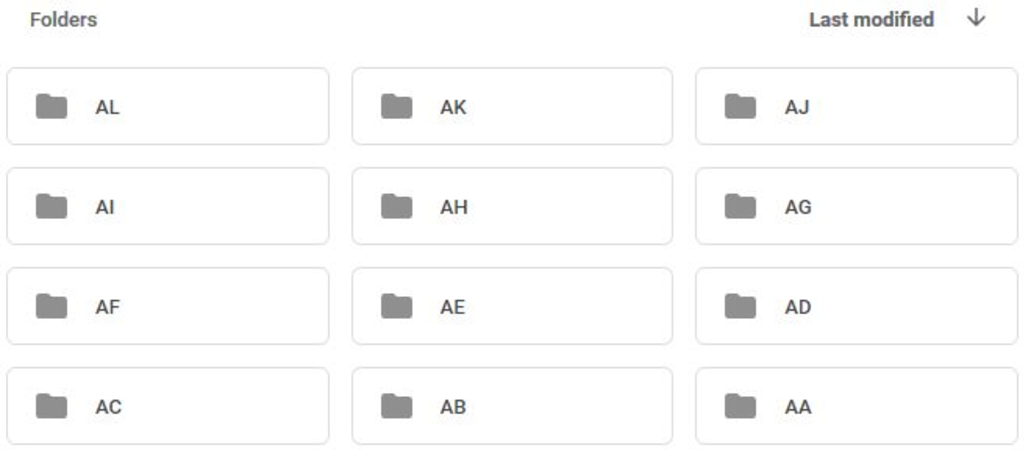
\includegraphics[scale=0.7]{Figures/wikidump.pdf}
\caption{Estructura de datos resultante al extraer un archivo de \textit{Wikipedia}.}
\label{fig:wikidump}
\end{figure}


\textbf{Obtención de datos.} El corpus de Wikipedia fue obtenido del sitio oficial (\url{https://dumps.wikimedia.org/eswiki/}). El corpus obtenido fue del mes de noviembre del año 2018. Estos archivos tienen una estructura específica y la forma recomendada de extraer sus contenidos es utilizando \emph{WikiExtractor} (\url{https://github.com/attardi/wikiextractor}). Esta herramienta permite realizar una extracción que filtra por un parámetro de mínimo de longitud del artículo. Se utilizó este parámetro para filtrar todos los artículos con menos de 10,000 caracteres.

Una vez finaliza la extracción del archivo --- la cual demora una cantidad no despreciable de horas --- se procede a leer y filtrar los documentos. En el caso de este trabajo se ignoraron todos los documentos después de haber acumulado 100 millones de tokens en los textos procesados. Se conservaron 10 millones de tokens adicionales para la validación de resultados.

\begin{table}
\begin{tabular}{| l | l |}

\hline
\textbf{Cadena de caracteres} & \textbf{Resultado tokenizado} \\
\hline
Hola, buenos días. & \texttt{xxbos xxmaj hola , buenos días} \\
HOLA!!! qué bueno verte & \texttt{xxbox xxmaj hola xxrep 3 ! qué bueno verte} \\
Mis audífonos son Sennheiser & \texttt{xxbos xxmaj mis audífonos son xxunk} \\
\hline

\end{tabular}
\caption{Muestras de tokenización utilizando \textit{spaCy} y técnicas de \textit{fastai}}
\label{tab:tokens}
\end{table}

\textbf{Tokenización.} La herramienta utilizada para este proceso fue spaCy (\url{https://spacy.io/}). Esta herramienta tiene soporte para más de 34 idiomas, entre los cuales se incluye el español. Además de esta herramienta se emplean técnicas adicionales como codificar caracteres repetidos o codificar palabras en mayúsculas --- ver tabla \ref{tab:tokens}.

\textbf{Definición de vocabulario.} Unos tokens son codificados como \texttt{xxunk} (token desconocido), esto es debido a la limitación de palabras únicas a codificar. El vocabulario fue limitado a 30,000 tokens únicos.

\begin{figure}
\centering
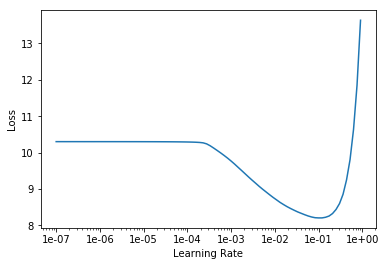
\includegraphics[scale=1]{Figures/lrfinder.png}
\caption{Ilustración de progreso de la función \texttt{lr\_find} de \textit{fast.ai}. Al momento de divergir el método deja de aumentar $\gamma$ y devuelve los resultados.}
\label{fig:lrfind}
\end{figure}

\textbf{Entrenamiento.} Luego tener los datos en el formato adecuado para entrenar el modelo se aplican las técnicas descritas en el capítulo \ref{Chapter3} sobre una red AWD LSTM. Previo a esto se encuentra un $ \gamma $ ideal y eso se hace aprovechando el método \texttt{lr\_find} (figura \ref{fig:lrfind}) de la librería de \emph{fastai} (\url{https://github.com/fastai/fastai}) que emplea el método descrito por \textcite{smith2017convergence}. Se aumenta $\gamma$ a medida que se recorren los ejemplos a entrenar. Si en algún momento diverge el aprendizaje se detiene el método y se imprime la gráfica. Se deberá querer elegir un $\gamma$ que no tenga riesgo de divergir el aprendizaje y que tampoco disminuya la velocidad del proceso. La elección adecuada de este hiper-parámetro en esta etapa es crucial para obtener un modelo en un tiempo razonable, ya que este modelo es el más grande --- en términos de parámetros y datos a procesar --- que requerirá entrenamiento. Vale la pena enfatizar que este proceso se realiza una \emph{única} vez y la definición de modelos clasificadores en un futuro podrá hacer uso del modelo entrenado originalmente.

\subsubsection{Resultados}

Para medir y reportar errores sobre LMs se utiliza la métrica de \textit{perplexity} \parencite{jurafsky2014speech}, la cual es análoga a la entropía. La entropía representa la cantidad de información que se tiene; \textit{perplexity} se puede ver como la cantidad de opciones que se tiene. ¿Qué significa esto? Que mientras menos opciones considere nuestro LM, más estable es y por lo tanto que modela mejor el lenguaje. Se calcula de la siguiente manera:

$$ perplexity = e^{loss} $$

En nuestro caso, se utiliza el valor de pérdida de los datos de validación.

\begin{table}
\centering
\begin{tabular}{|l|l|l|}
\hline
Modelo & Error en validación & \textit{Perplexity} \\
\hline
AWD LSTM & 3.140521 & \textbf{23.1038} \\
QRNN & 3.193912 & 24.2884 \\
\hline
\end{tabular}
\caption{Resultados de los modelos entrenados. La métrica que se utiliza para comparar entre los modelos es \textit{perplexity} la cual indica y representa qué tantas opciones se tienen para la siguiente palabra.}
\label{tab:modresults}
\end{table}

Se entrenaron dos modelos de RNN, uno fue basado directamente de la arquitectura y estrategias de AWD LSTM  y el otro modelo basado en la arquitectura QRNN. Los resultados se muestran en la tabla \ref{tab:modresults}. Sin embargo esta tabla no cuenta la historia completa. El modelo QRNN demoró menos en su entrenamiento de forma no insignificante tomando 13\% menos en entrenarse con resultados muy comparables a los de la red AWD LSTM.

\begin{table}
\centering
\begin{tabular}{|l|l|}
\hline
\textbf{Modelo} & \textbf{\textit{Perplexity}} \\
\hline
Transformer-XL \parencite{dai2019} & \textbf{18.3} \\
\hline
AWD LSTM (propio) & \textbf{23.1038} \\
QRNN (propio) & 24.2884 \\
Activation Mem. \parencite{rae2018} & 29.2 \\
RNN \parencite{goldszmidt2018} & N/A (34\% prec.) \\
RNN \parencite{ingham2018} & 36.1473 \\
\hline

\end{tabular}
\caption{Comparación de LMs con modelos del estado del arte en inglés y modelos de referencia para el español. Menor \textit{perplexity} es mejor. Separamos el modelo \textit{Transformer-XL} ya que utiliza otra arquitectura y está presente en la tabla solamente como referencia al mejor resultado al momento de haber escrito este trabajo.}
\label{tab:lmcomp}
\end{table}

En la tabla \ref{tab:lmcomp} se aprecian distintos LMs los cuales fueron entrenados en distintos datasets. El modelo Transformer-XL \parencite{dai2019} utiliza la nueva tendencia de finales del 2018 y principios de 2019 de usar transformadores en lugar de RNNs, así como propone Google con BERT. El modelo de \textit{Activation Memory} \parencite{rae2018} es un modelo de referencia que utiliza la arquitectura de una RNN simplificando un sub-conjunto de sus parámetros. Los otros dos modelos han sido modelos previamente entrenados con el propósito de ser usados para tareas clasificación en español con ULMFiT. Los datos presentados para los modelos propios fueron el valor de pérdida en un set de validación de 100 millones de tokens elegidos al azar de \textit{Wikiepedia}.

Aunque hay argumentos en contra de usar \textit{perplexity} para comparar LMs de distintos lenguajes o que usan distintos vocabularios \parencite{chen1998evaluation}, se debe tener un marco de referencia. Los modelos con propósitos de usar ULMFiT fueron entrenados de una forma muy similar al propio y son las comparaciones más directas por ser LMs del idioma español.


\subsubsection{Recursos utilizados para entrenamiento}

\textbf{Costo monetario.} Para esta fase de entrenamiento se recurre a los servicios de \textit{Google Cloud} (\href{https://cloud.google.com/free}{https://cloud.google.com}) los cuales son ofrecidos con un beneficio de 300 USD para utilizar durante el primer año. No es necesario ser estudiante o profesor para gozar de este beneficio. Teniendo estos recursos disponibles se optó por utilizar una instance de cómputo \emph{n1-highmem-4} (\url{https://cloud.google.com/compute/docs/machine-types}) la cual cuenta con	el siguiente hardware para el entrenamiento:

%\pagebreak

\begin{itemize}
\item Intel Xeon (Skylake) 4 vCPUs
\item 26 GB de memoria (RAM)
\item nVIDIA V100 GPU -- 16 GB de memoria
\end{itemize}

Lo primordial cuando se trata de entrenamiento de RNNs es la capacidad de cómputo de la GPU. La \textbf{V} en el modelo V100 indica que es de la última generación a la fecha de esta tesis y provee una ventaja significativa comparada con una K80 o P100.

\textbf{Costo de recursos.} El costo total resultante después de entrenar un modelo inicial y funcional llegó a \$ 60.20 USD. Esto fue cubierto por los créditos iniciales ofrecidos por Google. También se debe considerar que este paso se debe realizar \emph{una sola vez} para cada lenguaje. En caso de querer utilizar el modelo entrenado en este trabajo, se podrá hacerlo y se podrá aplicar a otros problemas de clasificación.

\textbf{Costo en tiempo.} Para entrenar los modelos de lenguaje con una estructura AWD LSTM, una época se demora alrededor de una hora. Después de 4 épocas se aproximan los resultados al estado del arte y debe decidirse cuando detener el entrenamiento sin perder la generalidad del sistema.

\subsection{Modelos clasificadores}

\textbf{Procesamiento de datos.} El conjunto de datos principales que se utilizó fue el de PAN17 \parencite{rangel2017overview}. Este conjunto de datos no es típico ya que consta de tuits de un grupo de usuarios. Cada uno de estos tuits --- 100 por usuario --- tiene asociado su usuario el cual tiene las etiquetas de edad y región asignadas. Por lo tanto se puede abordar el problema de distintas formas; se puede tomar cada tuit individual y predecir el género y la región individualmente, sumando después las probabilidades para obtener un veredicto final para el autor o se pueden concatenar los tuits del autor y realizar una solo predicción sobre ese texto completo del autor. Para este trabajo se utilizó cada tuit individual con el fin de poder tener un alcance mayor sobre la tarea de perfilación de autores sobre textos informales.

\begin{table}
\centering
\rowcolors{1}{gray!25}{white}
\begin{tabular}{| p{3cm} | p{9.5cm} |}
\hline
\textbf{Estado del texto} & \textbf{Resultado} \\
\hline
Original & \texttt{\#igualdaddegenero y \#mediosdecomunicacion http://t.me/ssbM} \\
Sin normalizar & \texttt{xxunk xxunk y xxunk xxunk xxunk} \\
Normalizado & \texttt{xxhashtag igualdad enero y xxhashtag medios comunica xxurl} \\
\hline
\end{tabular}
\caption{Ejemplificación de normalización de textos informales obtenidos del dataset PAN17 para la tarea de perfilación de autores. El proceso de normalización permite extraer información de los \textit{tokens} que son menciones de usuario y \textit{hashtags}. En la tabla se aprecia un ejemplo real con drásticos cambios dependiendo de procesamiento.}
\label{tab:pan17preproc}
\end{table}

\textbf{Pre-procesamiento y tokenización.} El procesamiento constó de normalizar los \textit{tokens} especiales de los textos (ver tabla \ref{tab:pan17preproc}); en particular se normalizaron las menciones de usuario y los \textit{hashtags}. Este proceso consistió en ordenar los \textit{tokens} del vocabulario del modelo pre-entrenado de \textit{Wikipedia} y buscar las instancias encontradas en los \textit{tokens} de interés. Luego de haber hecho esto, anteponer un \textit{token} especial que indique que se encontraba ahí originalmente, por ejemplo \texttt{xxhashtag}. Se tokenizan los datos de la misma manera en que se tokenizaron los datos en la fase de modelo de lenguaje; utilizando \textit{spaCy}.

\textbf{Afinación de LM.} Después de haber entrenado el modelo de lenguaje se procede a una fase de afinación \parencite{howard2018}. Se emplean las técnicas descritas en el capítulo \ref{Chapter3} para poder afinar el modelo. Este proceso se realiza con los datos de la tarea en específico. Se adapta el formato de los datos de clasificación a datos para entrenamiento de un LM y se afina el modelo para textos de este dominio específico. Sobre la métrica de \textit{perplexity} o la precisión no se pone mayor énfasis, lo importante será que la estructura general de los textos y el vocabulario que se use refleje los datos reales del problema específico.

\begin{comment}
resultados en afinamiento de lm aca. grafica? tabla?
\end{comment}

\textbf{Entrenamiento de los modelos clasificadores.} Al tener el LM afinado se procede a entrenar un clasificador. Este proceso es descrito en la sección \ref{sec:nlpprocess}. A continuación se detallan las decisiones tomadas.

\begin{figure}
\centering
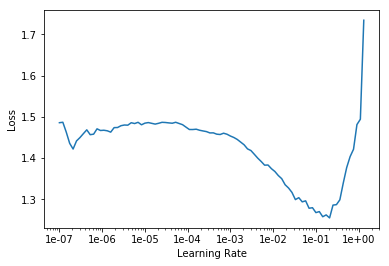
\includegraphics[scale=1]{Figures/clas_lrfinder.png}
\caption{Evolución de la pérdida conforme se cambia la tasa de aprendizaje en el clasificador. Al igual que con el LM, se deberá elegir un valor óptimo para mayor eficiencia.}
\label{fig:claslr}
\end{figure}

\textbf{Entrenamiento del clasificador.} Antes de comenzar con el entrenamiento se deben elegir los hiper-parámetros adecuados. Primero se eligió un peso para los parámetros de \textit{dropout} (basado en pruebas empíricas) y después se eligió un $\gamma$ óptimo basado en la herramienta de \texttt{lr\_find} (figura \ref{fig:claslr}). Los valores elegidos fueron \texttt{dropout = 0.3} y un $\gamma$ inicial con valor de \texttt{1e-2}. Se habla de un $\gamma$ inicial ya que en el entrenamiento del modelo clasificador se aplica el concepto de usar un $\gamma$ cíclico \parencite{smith2017convergence} abordado en el capítulo \ref{Chapter3}.

\begin{figure}
\centering
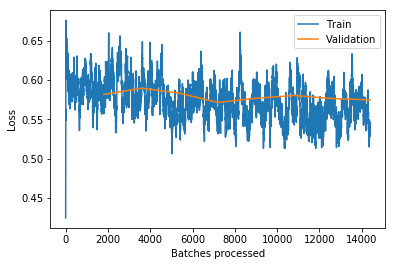
\includegraphics[scale=1]{Figures/clas_epochs.png}
\caption{Avance de pérdida conforme avanzan las épocas de entrenamiento. Menor es mejor.}
\label{fig:clasepochs}
\end{figure}

El entrenamiento de un clasificador con pocos datos no deberá tomar mucho tiempo y los resultados deberán ser satisfactorios aplicando los temas expuestos en este trabajo. En la figura \ref{fig:clasepochs} se puede apreciar como la evolución de pérdida avanza lentamente a través de las épocas y converge en un valor después de un número de épocas relativamente bajo. Sin embargo, es posible continuar con el entrenamiento hasta lidiar con \textit{overfitting}. Este problema surge cuando se han afinado tanto los parámetros del modelo que el proceso de \textit{backpropagation} empieza a ajustarse conforme solamente los datos de entrenamiento y no el problema en sí. La manera más fácil de detectar este fenómeno es con la comparación de resultados sobre la función de pérdida de los datos de entrenamiento con los datos de evaluación. Si el valor de pérdida para ambos conjuntos de datos disminuye significa que el entrenamiento se está realizando con éxito. Si en algún momento el valor de pérdida para los datos de entrenamiento continua disminuyendo pero al mismo tiempo el valor de pérdida para los datos de validación aumenta significa que ya no estamos obteniendo resultados que puedan ser generalizados a datos no antes vistos.

\begin{comment}
grafica de overfitting
\end{comment}



\section{Resultados}

Se ha dicho que para RNNs y técnicas de aprendizaje profundo no han tenido el mismo éxito que en otras tareas debido a la dificultad que un modelo de aprendizaje profundo tiene al aprender la cantidad de parámetros inmensa con pocos datos \parencite{zampieri2017, malmasi2016discriminating}. Esta tarea es por lo tanto ideal para poder determinar la capacidad real la transferencia de aprendizaje en NLP y sobre todo cuando las instancias de aprendizaje son limitadas.

Los datos y resultados en referencia a predicción de región y género provienen del reporte de la competencia PAN17 \parencite{rangel2017overview} y proveen un contexto para la tarea del trazo de perfiles de autores. Debido a que los conjuntos de datos de pruebas son los mismos, las comparaciones se podrán hacer de forma directa. Se realiza una comparación con datos exclusivamente del idioma español. Los modelos a comparar son los siguientes:

\begin{itemize}
\item TF-IDF + CNN \parencite{schaetti2017author}
\item RNN \parencite{kodiyan2017author}
\item AVG DNN \parencite{franco2017author}
\item CNN + RNN + Attention \parencite{miura2017author}
\end{itemize}

Para estos resultados se utiliza la métrica usada en la competencia PAN17 la cuál es:

% \: es un espacio de mediana distancia

$$ Acc_{cat} = \frac{Predicciones\: correctas}{Total\: de\: predicciones} $$

Donde $cat$ es la categoría sobre la cual se está prediciendo. Las predicciones son aplicadas sobre los datos de validación, los cuales fueron segmentados por el equipo organizador de PAN17 los cuales cuenta con 2,800 autores, cada uno asociado a 100 tuits.

\subsection{Predicción de género}

La predicción de género sobre un texto anónimo se realizó basado en datos de tuits. La clasificación se llevó a cabo en dos niveles. Se realizó una predicción a nivel de tuit individual y una predicción a nivel de autor.

\begin{table}
\centering
\begin{tabular}{r | c c}
\multicolumn{3}{c}{\textbf{Referencia}} \\
\textbf{Predicción} & Femenino & Masculino \\
\hline
Femenino & 83110 & 49573 \\
Masculino & 56890 & 90427 \\
\end{tabular}
\caption{Matriz de confusión de resultados sobre predicción de género en tuits individuales.}
\label{tab:gender_indvtweet}
\end{table}

En la tabla \ref{tab:gender_indvtweet} se aprecian los resultados de las predicciones sobre tuits individuales. La evaluación de la métrica con estos datos sería entonces:

$$ Acc_{gender\_idv} = \frac{173,537}{280,000} = 0\text{.}6198 $$

\begin{table}
\centering
\begin{tabular}{r| c c}
\multicolumn{3}{c}{\textbf{Referencia}} \\
\textbf{Predicción} & Femenino & Masculino \\
\hline
Femenino & 963 & 283 \\
Masculino & 437 & 1117 \\
\end{tabular}
\caption{Matriz de confusión de resultados de predicciones por autor.}
\label{tab:gender_authtweet}
\end{table}

La predicción sobre los autores es basada en las predicciones sobre tuits individuales. Esto resulta en una suma ponderada de las predicciones individuales descrita como
\[ \phantom{,}\hat{p}_a (\mathbf{X}) = \max \sum_{n = 1}^{100} p(X_n), \]
donde $\mathbf{X}$ representa una matriz de probabilidades; las filas representan tuits individuales y las columnas las probabilidades de que el tuit pertenezca a la categoría de esa columna (p.e. el género femenino).

Dada la anterior tenemos la tabla \ref{tab:gender_authtweet} y un resultado de
\[ \phantom{.}Acc_{gender} = 0\text{.}7429. \]

La sumatoria ponderada resulta en un sistema similar a un ensamble de modelos los cuales toman prioridad según la confianza que tengan en su predicción. Debido a esto, el resultado aumenta en la métrica considerablemente.

\begin{table}
\centering
\rowcolors{2}{gray!25}{white}
\begin{tabular}{p{9.5cm} p{3cm}}
\textbf{Modelo} & \textbf{Resultado} \\
\hline
TF-IDF + CNN \tblshort\parencite{schaetti2017author} & 0.7150 \\
RNN \tblshort\parencite{kodiyan2017author} & 0.7217 \\
RNN + Transfer Learning (propio) & 0.7429 \\
AVG DNN \tblshort\parencite{franco2017author} & \textbf{0.7721} \\
\hdashline
\rowcolor{white}
CNN + RNN + Attention \tblshort\parencite{miura2017author} & \textbf{0.8118} \\

\end{tabular}
\caption{Comparación de modelos de aprendizaje profundo en la tarea de predicción de género --- mayor es mejor. El modelo de \tblshort\textcite{miura2017author} se separa ya que es un ensamble de modelos y no se puede hacer una comparación directa.}
\label{tab:pan17gender}
\end{table}

Al comparar el modelo propio con los modelos de aprendizaje profundo presentados en la competencia PAN17 (tabla \ref{tab:pan17gender}) se puede apreciar que los resultados obtenidos son del estado del arte para RNN, siendo solamente superado por un AVG DNN y un ensamble de CNN, RNN y elementos de atención.

\subsection{Predicción de región}

La predicción de género sobre un texto anónimo se realizó basado en datos de tuits. La clasificación se llevó a cabo en dos niveles. Se realizó una predicción a nivel de tuit individual y una predicción a nivel de autor.

\begin{table}
\centering
\begin{tabular}{r | c c c c c c c}
\multicolumn{3}{c}{\textbf{Referencia}} \\
\textbf{Predicción} & AR & CL & CO & MX & PE & ES & VZ\\
\hline
AR & 22,610 & 3,013 & 3,147 & 2,220 & 3,783 & 2,558 & 2,188 \\
CL & 3,064 & 21,058 & 2,988 & 3,034 & 3,760 & 2,599 & 2,454 \\
CO & 3,435 & 2,993 & 20,007 & 4,401 & 4,251 & 2,746 & 3,696 \\
MX & 2,554 & 3,429 & 3,977 & 18,803 & 4,173 & 3,681 & 3,616 \\
PE & 2,992 & 3,780 & 3,544 & 3,542 & 17,812 & 2,552 & 2,605 \\
ES & 3,331 & 3,565 & 3,519 & 5,131 & 3,662 & 23,722 & 3,689 \\
VZ & 2,014 & 2,162 & 2,818 & 2,869 & 2,559 & 2,142 & 21,752 \\
\end{tabular}
\caption{Matriz de confusión de resultados sobre predicción de región en tuits individuales.}
\label{tab:region_indvtweet}
\end{table}

De la misma manera que con las predicciones de género, en la tabla \ref{tab:region_indvtweet} se aprecian los resultados de las predicciones sobre tuits individuales. La evaluación de la métrica con estos datos --- siendo esta solo indicativa --- sería entonces la siguiente:

$$ Acc_{region\_idv} = \frac{145,764}{280,000} = 0\text{.}5206 $$

\begin{table}
\centering
\begin{tabular}{r| c c c c c c c}
\multicolumn{3}{c}{\textbf{Referencia}} \\
\textbf{Predicción} & AR & CL & CO & MX & PE & ES & VZ\\
\hline
AR & 381 & 5 & 7 & 5 & 14 & 1 & 7 \\
CL & 2 & 370 & 2 & 3 & 4 & 1 & 1 \\
CO & 2 & 3 & 367 & 10 & 9 & 3 & 8 \\
MX & 3 & 5 & 4 & 364 & 9 & 3 & 9 \\
PE & 4 & 7 & 8 & 3 & 353 & 3 & 4 \\
ES & 5 & 5 & 8 & 13 & 4 & 388 & 17 \\
VZ & 3 & 5 & 3 & 2 & 7 & 1 & 354 \\
\end{tabular}
\caption{Matriz de confusión de resultados de predicción de región por autor.}
\label{tab:region_authtweet}
\end{table}

La predicción sobre los autores basada en la suma ponderada tenemos la tabla \ref{tab:region_authtweet} y un resultado de
\[ \phantom{.}Acc_{region} = 0\text{.}9207. \]

La sumatoria ponderada resulta en un resultado mucho mayor que el de las predicciones individuales. Esto puede deberse a dos cosas:

\begin{itemize}
\item Muchos tuits son muy limitados en su número de caracteres por lo que algunos no revelarán mucha información acerca del autor por sí solos.
\item La cobertura de vocabulario con palabras regionales disminuye por lo que algunos tuits individuales con palabras claves no proveen mucha información.
\end{itemize}

\begin{table}
\centering
\rowcolors{2}{gray!25}{white}
\begin{tabular}{p{9.5cm} p{3cm}}
\textbf{Modelo} & \textbf{Resultado} \\
\hline
TF-IDF + CNN \tblshort\parencite{schaetti2017author} & \textbf{0.9336} \\
RNN \tblshort\parencite{kodiyan2017author} & 0.9143 \\
RNN + Transfer Learning (propio) & 0.9207 \\
AVG DNN \tblshort\parencite{franco2017author} & 0.9000 \\
\hdashline
\rowcolor{white}
CNN + RNN(Att.) \tblshort\parencite{miura2017author} & \textbf{0.9271} \\

\end{tabular}
\caption{Comparación de modelos de aprendizaje profundo en la tarea de predicción de región --- mayor es mejor. El modelo de \tblshort\textcite{miura2017author} se separa ya que es un ensamble de modelos y no es posible hacer una comparación directa.}
\label{tab:pan17region}
\end{table}

Nuevamente se comparan los resultados con los modelos de aprendizaje profundo de PAN17 (tabla \ref{tab:pan17region}). Una combinación de TF-IDF y CNN \parencite{schaetti2017author} logró clasificar de la mejor manera; el modelo propio obtiene la segunda mejor precisión en modelos simples y la tercera considerando el ensamble de modelos CNN y RNN de \textcite{miura2017author}.

\subsection{Predicción sobre textos formales}

Los experimentos se repiten sobre textos formales usando los datos de SpanText \parencite{villegas:2014:CACIC}. Los datos de referencia y comparación se obtuvieron directamente de la publicación del conjunto de datos.


% Chapter 6

\chapter{Conclusiones}

\label{Chapter6} % For referencing the chapter elsewhere, use \ref{Chapter6}

En este capítulo se presentan las conclusiones obtenidas a partir del trabajo de investigación y los resultados encontrados.

\section{Conclusiones}

El campo de Deep Learning ha mostrado mucha promesa en los últimos años, pero el área de NLP no ha mostrado tanta promesa sino hasta el último año. En este trabajo se busca fomentar y profundizar más la penetración que han tenido estas técnicas en el área, tanto en sectores industriales como académicos.

Para plantear las conclusiones de este trabajo, se deberá recordar los objetivos principales mencionados en un comienzo. Se pretendía plantear un sistema competitivo a niveles del estado del arte que no requiriera ingeniería de características sobre los textos. Un modelo que no requiriera expertiz en el campo de la lingüística para ser diseñado; un modelo que no necesitara tantos ejemplos de entrenamiento para generalizar y desempeñarse bien la tarea asignada. LEFTy cumple con estos objetivos de forma elegante y novedosa aplicando \textit{transfer learning} a la tarea de perfilamiento de autores en el área de NLP.

Este concepto permite abrir muchas puertas y se ha demostrado que no sólo aplica para el área de visión artificial con muchas publicaciones en el último año de laboratorios grandes como OpenAI, fastai, Google, Deep Mind, etc. La promesa que trae esta técnica a NLP, permitiría aplicarse a una infinidad de tareas sin depender de muchos ejemplos, justo como se pudo apreciar con los resultados presentados sobre textos formales.

Sin embargo, \textit{transfer learning} tiene compromisos que se deben tomar en cuenta, a pesar de todas las ventajas que provee. Una de ellas es no cambiar la estructura del modelo pre-entrenado de una manera muy significativa sin el riesgo de una pérdida catastrófica del aprendizaje general con el que se cuenta. Lo anterior lleva también a la conclusión que se debe tener mucho cuidado al afinar un modelo general a una tarea específica en NLP, ya que se tiene el mismo riesgo si se entrena de manera desenfrenada.

En este trabajo se reiteran algunas técnicas de afinamiento de modelos, tanto para modelos de lenguaje como para modelos clasificadores de una tarea final, reproduciendo de manera parcial los resultados presentados por \citeauthor{howard2018}.

Los resultados presentados en el capítulo \ref{Chapter5} de este trabajo compiten con los modelos del estado del arte y con gente que se ha dedicado por años al estudio de NLP, lingüística y su intersección como ciencias. Esto demuestra que no se debe ser persona experta para aprovechar el poder del deep learning.

Se presentó un modelo de lenguaje del idioma español que puede ser utilizado para una cantidad ilimitada de tareas y se hizo público para que pueda ser aprovechado por la comunidad científica en esta área; este ha sido descargado más de 30 veces al momento de la publicación de este trabajo.

El modelo publicado también provee la ventaja de permitir una reducción de costos al entrenar modelos clasificadores futuros, ya que el mayor costo presentado en este trabajo fue el del entrenamiento del modelo de lenguaje general entrenado sobre datos de Wikipedia. Este hecho promete que el uso de Deep Learning no sea prohibitivo para compañías e individuos que no tienen acceso a poder computacional masivo o incluso ilimitado como algunas compañías, lo que se considera una contribución muy valiosa a la comunidad.

\section{Trabajo futuro}

Las estrategias, técnicas y tecnologías utilizadas en este trabajo muestra un balance entre obtener resultados del estado del arte y realizar la tarea sin sobrellevar costos prohibitivos. Debido a esto, algunas técnicas no fueron utilizadas debido a limitaciones económicas o temporales y una sección de trabajo futuro es necesaria.

Asimismo, debido a que el desarrollo en esta área tiene un ritmo muy acelerado, durante la elaboración de este trabajo se realizaron múltiples publicaciones con nuevos aportes a la comunidad científica que pueden ser de mucho valor para la aplicación específica descrita en este proyecto.

A continuación se plantea el trabajo futuro a considerar:

\begin{itemize}

\item La adición más simple que se podría hacer con el trabajo realizado es utilizar LSTMs bidireccionales. En este caso en particular significaría entrenar un modelo que evalúe los tuis con el orden inverso de las palabras y realizar un ensamble de los modelos resultantes.

\item \textcite{radford2019language} han mostrado que utilizar textos más diversos y en mayores cantidades para el entrenamiento de modelos de lenguaje puede resultar en una ventaja adicional, no sólo en ese modelo en particular sino en las tareas específicas para las que después se utilizará el sistema pre-entrenado.

\item El uso de una nueva estructura llamada transformador ha tomado un auge en el año 2018 y 2019 y ha presentado nuevos resultados del estado del arte. En algunas ocasiones ha superado por un margen elevado al resultado a vencer. Esto indica que puede aportar mucho valor usar una estructura de trasnformador en lugar de una de LSTM. Los transformadores proveen ventajas como la posibilidad de ser entrenados en modalidades paralelas. Sin embargo, muchos resultados han necesitado de mucho poder computacional por lo que puede llegar a ser prohibitivo su uso.

\item En este trabajo se mostró que el pre-procesamiento de los textos antes de ser alimentados al modelo no es perfecto, por lo que se deben explorar formas de refinar esto. En particular, la normalización y conservación del aspecto semántico de los textos, especialmente los informales, requerirán de mayor esfuerzo y experimentación.

\item Para este trabajo se clasificaron los tuits individualmente, sin embargo existía la posibilidad de utilizar concatenación de textos y evaluar sobre el texto resultante para cada autor. Se podría usar este abordamiento al problema y evaluar si se obtiene mejor desempeño. Esto tendría el propósito de mejorar la posición en una competencia y no de avanzar el campo en esta tarea en específico.

\item Muchos avances se han realizado en los últimos años con respecto a modelos multi-tarea (multitask) --- que son modelos que tienen la capacidad de realizar múltiples predicciones, cada una de una tarea independiente. Tener solamente un modelo resultaría en menores tiempos de inferencia y menores requerimientos de memoria en el servidor donde se monte el sistema de predicción.


\end{itemize}



%----------------------------------------------------------------------------------------
%	THESIS CONTENT - APPENDICES
%----------------------------------------------------------------------------------------

\appendix % Cue to tell LaTeX that the following "chapters" are Appendices

% Include the appendices of the thesis as separate files from the Appendices folder
% Uncomment the lines as you write the Appendices

% Appendix A

\chapter{Analisis exploratorio de datos} % Main appendix title

\label{AppendixA} % For referencing this appendix elsewhere, use \ref{AppendixA}

\section{Datos utilizados para la clasificación}

The color of links can be changed to your liking using:

{\small\verb!\hypersetup{urlcolor=blue}!}

%\include{Appendices/AppendixB}
%\include{Appendices/AppendixC}

%----------------------------------------------------------------------------------------
%	BIBLIOGRAPHY
%----------------------------------------------------------------------------------------

\nocite{*}
\printbibliography[heading=bibintoc]

%----------------------------------------------------------------------------------------

\end{document}  
